\subsubsection{Settings}

The settings sketch can be seen in \cref{SettingsScreen} and are divided into 2 sketches. The left sketch show the list of settings, and the right sketch show the list of settings, with a specific sketch expanded.

\begin{figure}[H]
	\centering
    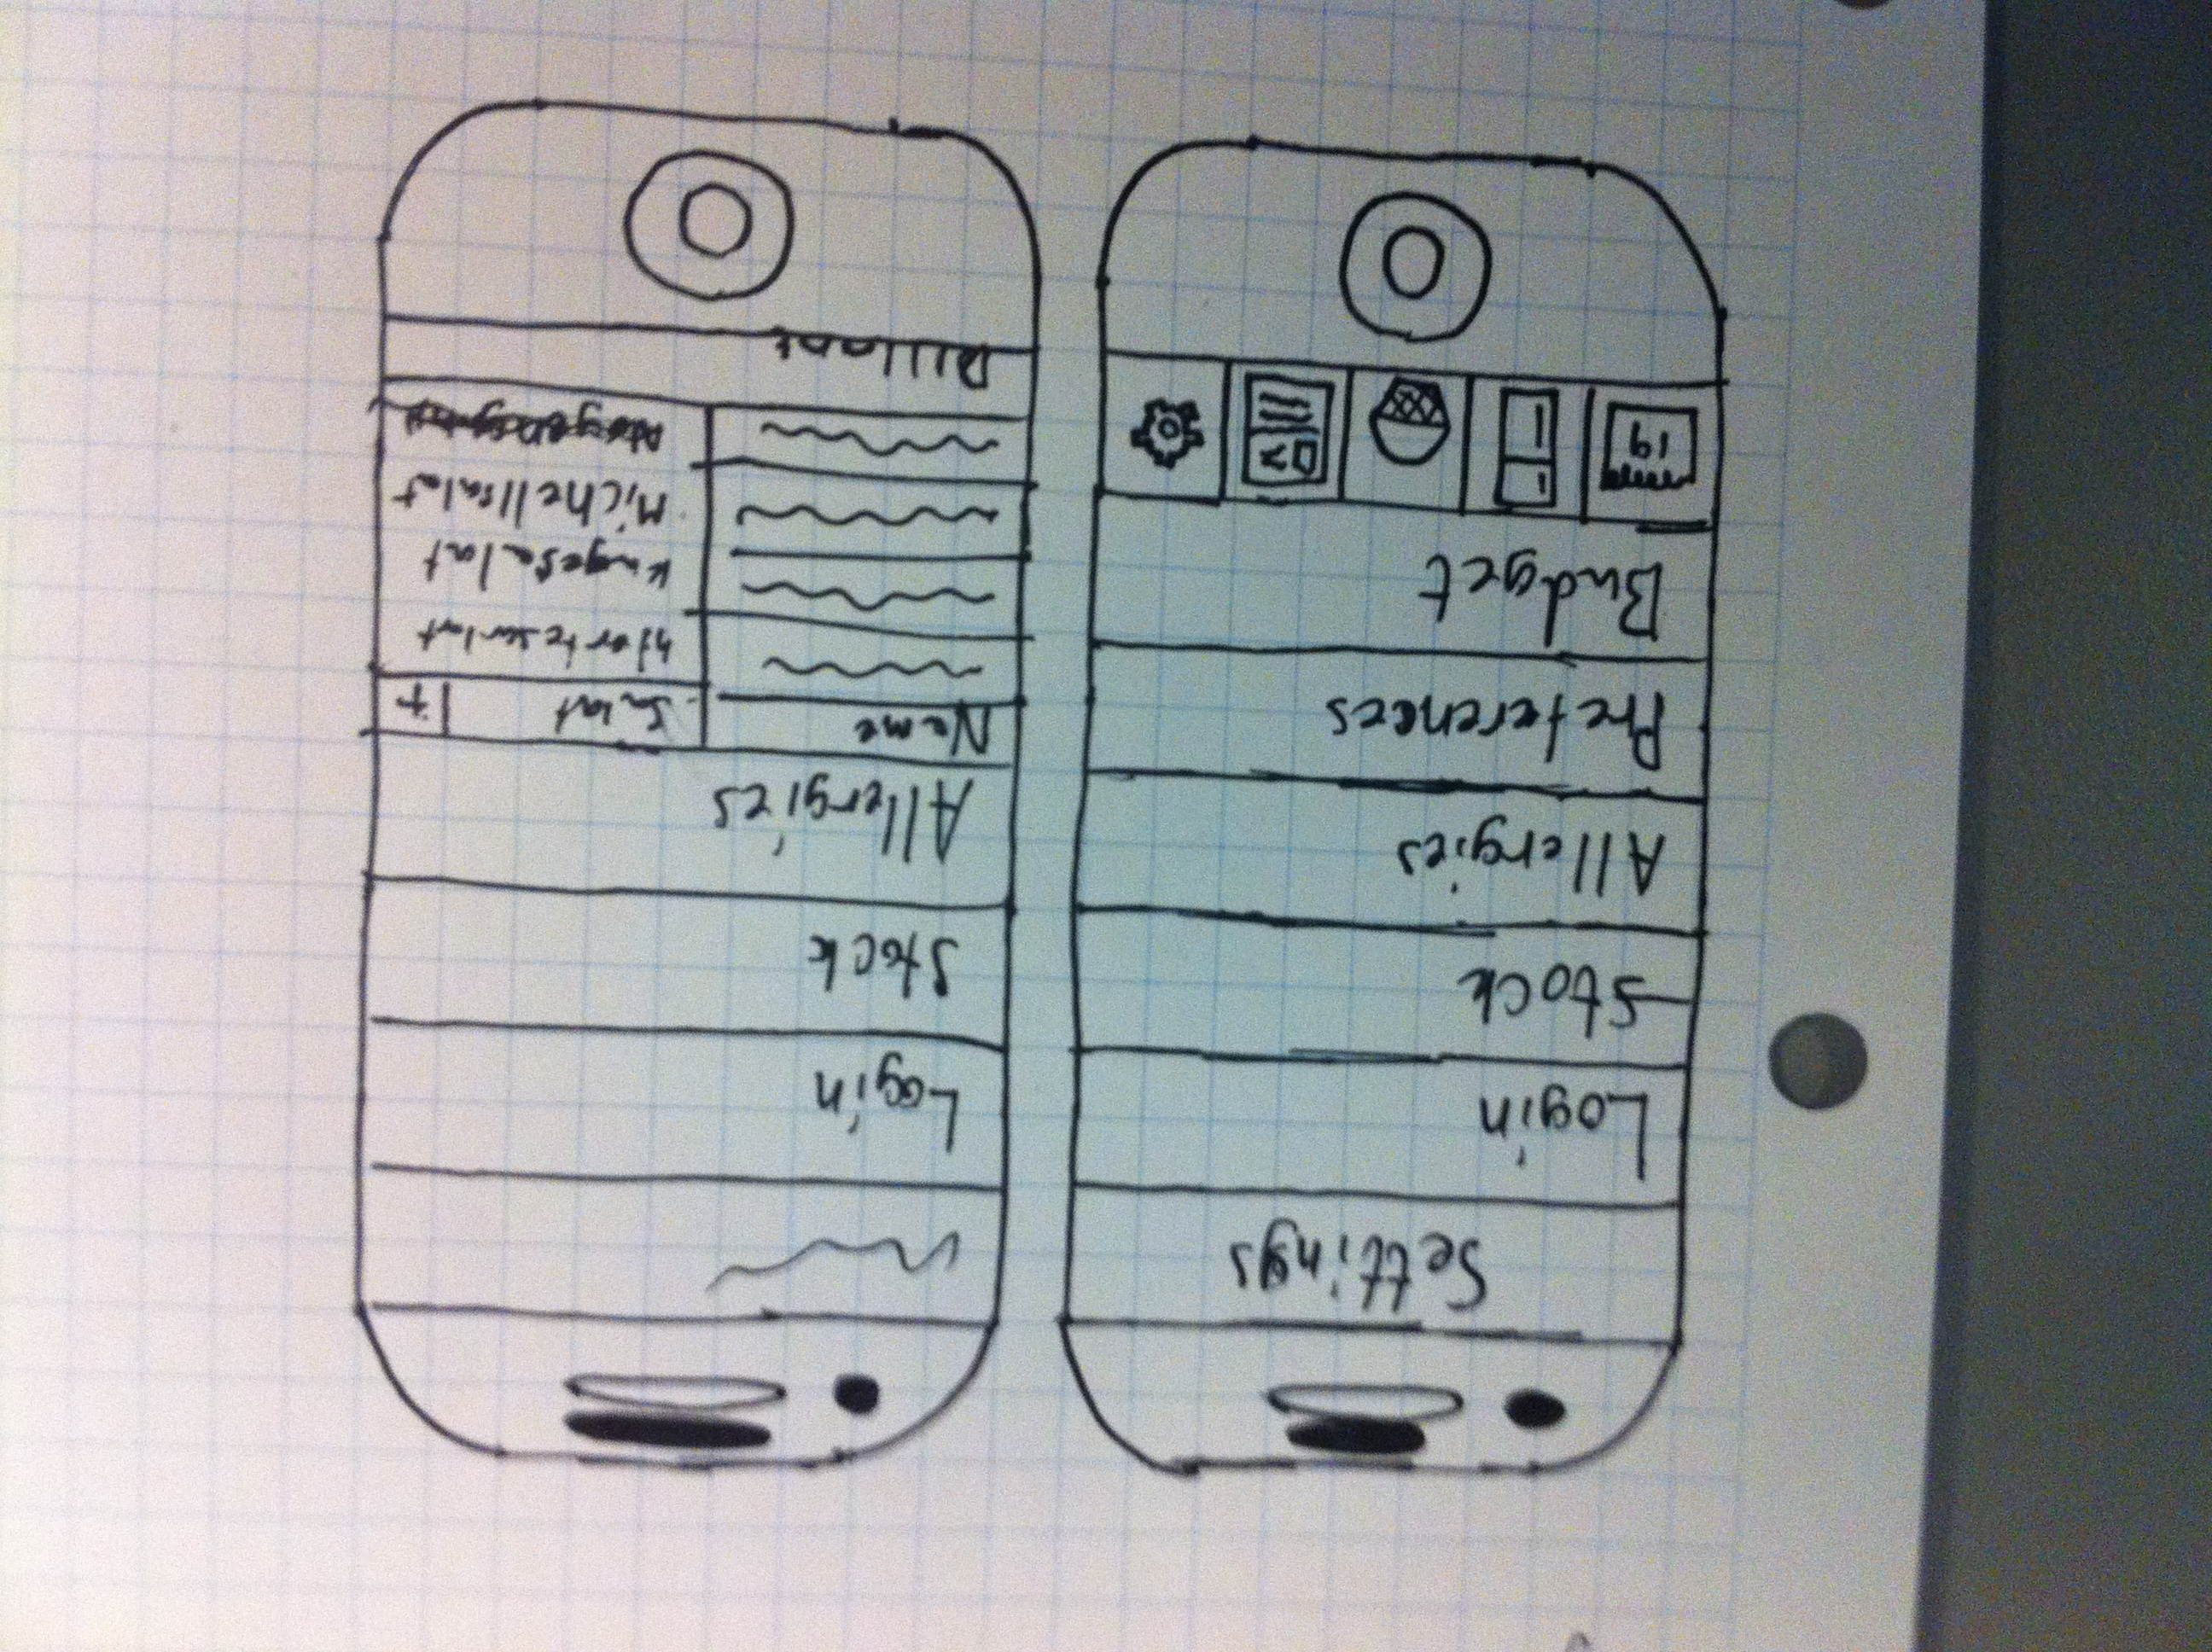
\includegraphics[width=0.5\textwidth]{Grafik/FoodPlanner/FinalSettingsSketch}
	\caption{This screen displays all of the settings in the program.}
	\label{SettingsScreen}
\end{figure}

\paragraph{Settings List} \label{SettingsList}

The setting list is the left sketch in \cref{SettingsScreen} and show a list of settings. The settings can be scrolled through, by swiping up and down, if more settings are needed than the screen can hold. The items shown in the sketch are just ideas for settings, and are just used to visualize the design idea. These are not all settings that will be incorporated in the program.

\paragraph{Expanded Settings List}

The right sketch in \cref{SettingsScreen} show the list of settings, as described in \cref{SettingsList}. Furthermore, this sketch has an expanded setting. This is because if a user click a setting,  it will expand, and show more information about this setting. In the sketch, allergies is expanded.

Expanding was chosen, because it would be consistent with the rest of the program, instead of other ideas that where discussed, for example a pop up. 